\documentclass{report}  % Specifies the document class
\usepackage[utf8]{inputenc}  % For UTF-8 encoding
\usepackage[top=3.5cm, left=3cm, right=3cm]{geometry}
\usepackage{booktabs}
\usepackage{fancyvrb}
\usepackage{xcolor}
\usepackage{float}
\usepackage{listings}
\usepackage{setspace}
\usepackage{graphicx}
\title{Houdini Tricks Writeup}  % Title of the document
\author{Huzaifa Patel}  % Author of the document
\date{\today}  % Date of the document


\lstset{ 
  frame=single,                   % Frame around the code
  breaklines=true,                % Line breaking
  basicstyle=\ttfamily,           % Font style
  backgroundcolor=\color{lightgray}, % Background color
  keywordstyle=\color{blue},      % Keywords style
  commentstyle=\color{green},     % Comments style
  stringstyle=\color{red}         % Strings style
}


\begin{document}  % Start of the document

\maketitle % Generates the title


\section{Verify Proper cgroup Functionality on Containers}

\large{
Docker containers can significantly impact the host system, particularly in terms of CPU usage. Unlike virtual machines (VMs), which have dedicated CPU resources and run their own operating systems, containers share the host's kernel and rely on the host’s CPU scheduler for processing power. This shared resource model makes container performance highly dependent on how the host allocates and schedules CPU time.

Docker uses control groups (cgroups) to enforce CPU resource limits and prioritize workloads, ensuring that no container consumes more CPU than allocated. The CPU scheduler adjusts dynamically based on factors like container priority, resource limits, and overall system load. However, it’s critical to ensure that cgroups are working as intended, as misconfigurations or failures could result in containers consuming excessive CPU resources, impacting system performance.

While cgroups offer powerful tools for resource management, there is a growing need for more empirical data on how cgroups perform under real-world workloads. Understanding how cgroups actually enforce CPU limits, particularly in complex multi-container environments, requires deeper analysis. Collecting data on the effectiveness and efficiency of cgroup settings under various conditions would provide valuable insights. Therefore, we provide two different tricks to verify proper cgroup functionality on containers.

The first trick is about setting cpu\_quota and cpu\_period to its default state, and running stress in the container. While the stress process is running, we use perf on the host to generate a flamegraph. Our rationale for conducting this trick is because setting `cpu\_quota` and `cpu\_period` to their default state allows the container to use as much CPU as needed, which can help us observe the container's natural CPU behavior under stress. This provides a baseline for comparison when different cgroup limits are applied. Linux kernel version 6.5.5 is used.
}

\begin{figure}[H]
    \centering
    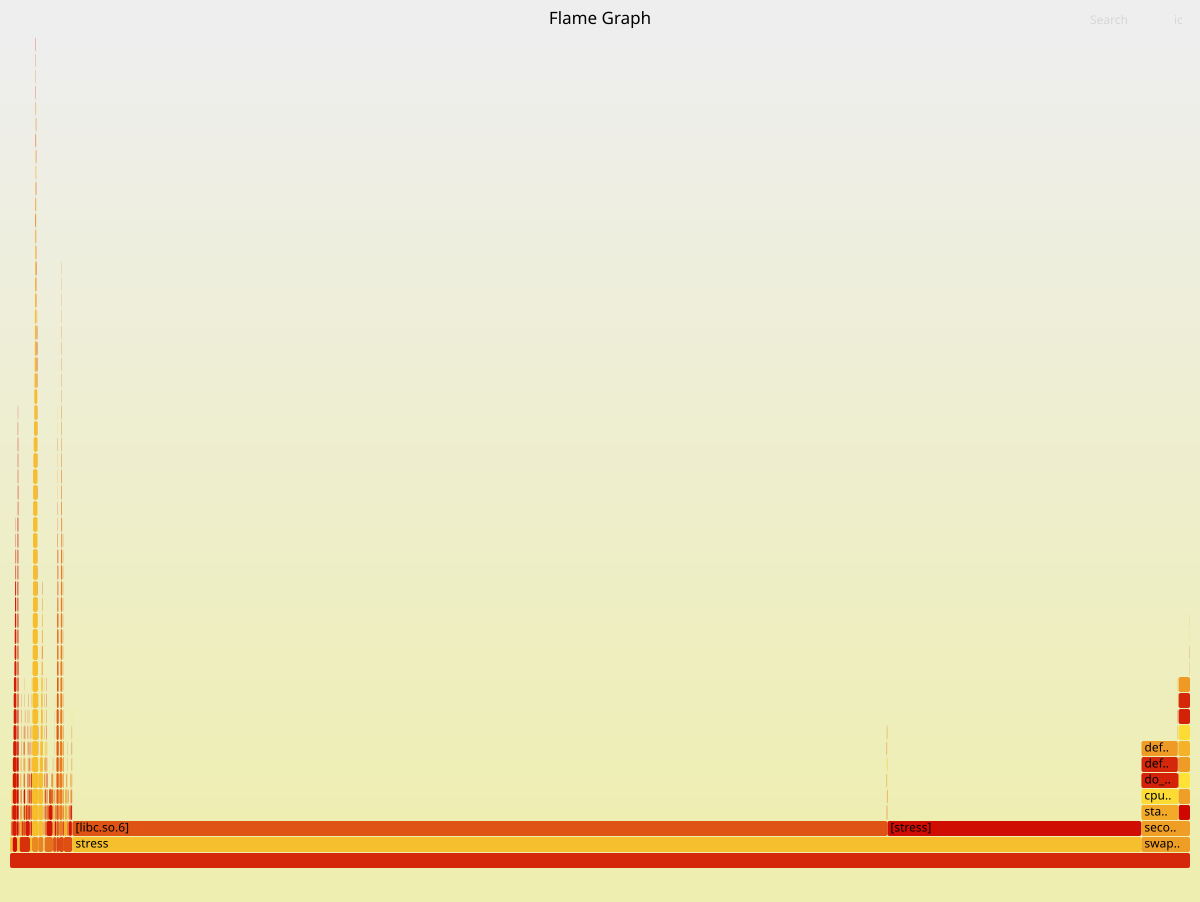
\includegraphics[width=\textwidth]{cpu_tricks/6.5.5/V1/flamegraph_20241017_092801.png}
    \caption{Flamegraph illustrating cpu\_quota and cpu\_period at its default state.}
    \label{fig:flamegraph}
\end{figure}


\large{
  The second trick involves configuring `cpu\_quota` to 50,000 and `cpu\_period` to 100,000. These parameters control how much CPU time a container can use within a given period. Specifically, setting `cpu\_quota` to 50,000 and `cpu\_period` to 100,000 means that the container is allowed to use up to 50\% of a single CPU core over a 100-millisecond window.

  This configuration ensures that the container can run tasks only for 50\% of the time in each scheduling period. If the container tries to exceed this limit, it will be throttled and forced to wait until the next scheduling period. This allows us to observe how the container behaves under constrained CPU conditions and how effectively the cgroup enforces this limitation.

  By using this setup, we can measure the container’s performance, responsiveness, and ability to handle workloads with limited CPU resources. Additionally, it helps us verify that the cgroup is accurately enforcing the CPU quota and preventing the container from exceeding its allocated CPU share. This is especially useful in multi-tenant environments where fair distribution of resources is critical to ensure that no single container negatively impacts the performance of other containers or the host system.
}

\begin{figure}[H]
    \centering
    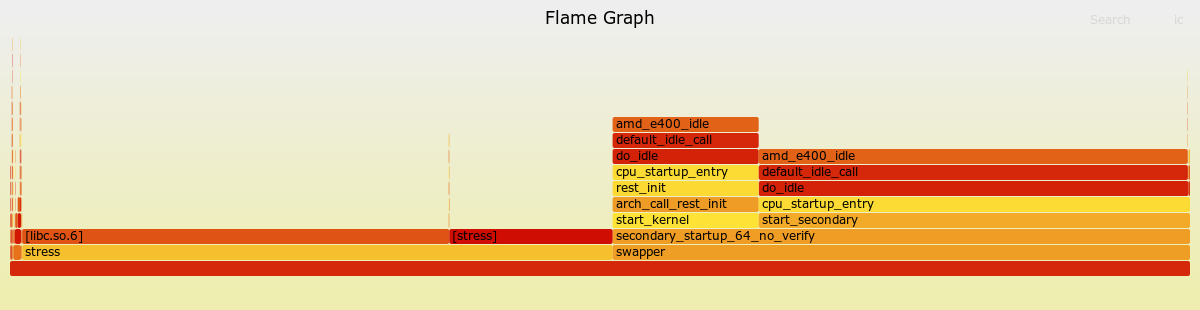
\includegraphics[width=\textwidth]{cpu_tricks/6.5.5/V1/flamegraph_20241022_175446.png}
    \caption{Flamegraph illustrating cpu\_quota and cpu\_period at 50,000 and 100,000, respectively}
    \label{fig:flamegraph}
\end{figure}


\large{
  The third trick tests whether cgroups abide by the cpuset\_cpus configuration placed during docker runtime. First, we set cpuset\_cpus to use only 1 CPU, more specifically the 0th CPU. Again, we run stress in the container. However, in the host, we run perf with only instrumenting the first, second, and third CPU. In total, the VM and container have four CPUs. With the results below, which was run on Linux kernel 6.5.5, we can see that the flamegraph does not have a stress process. This indicates that cgroups was only using the zeroth CPU to run stress in the container. 
}

\begin{figure}[H]
    \centering
    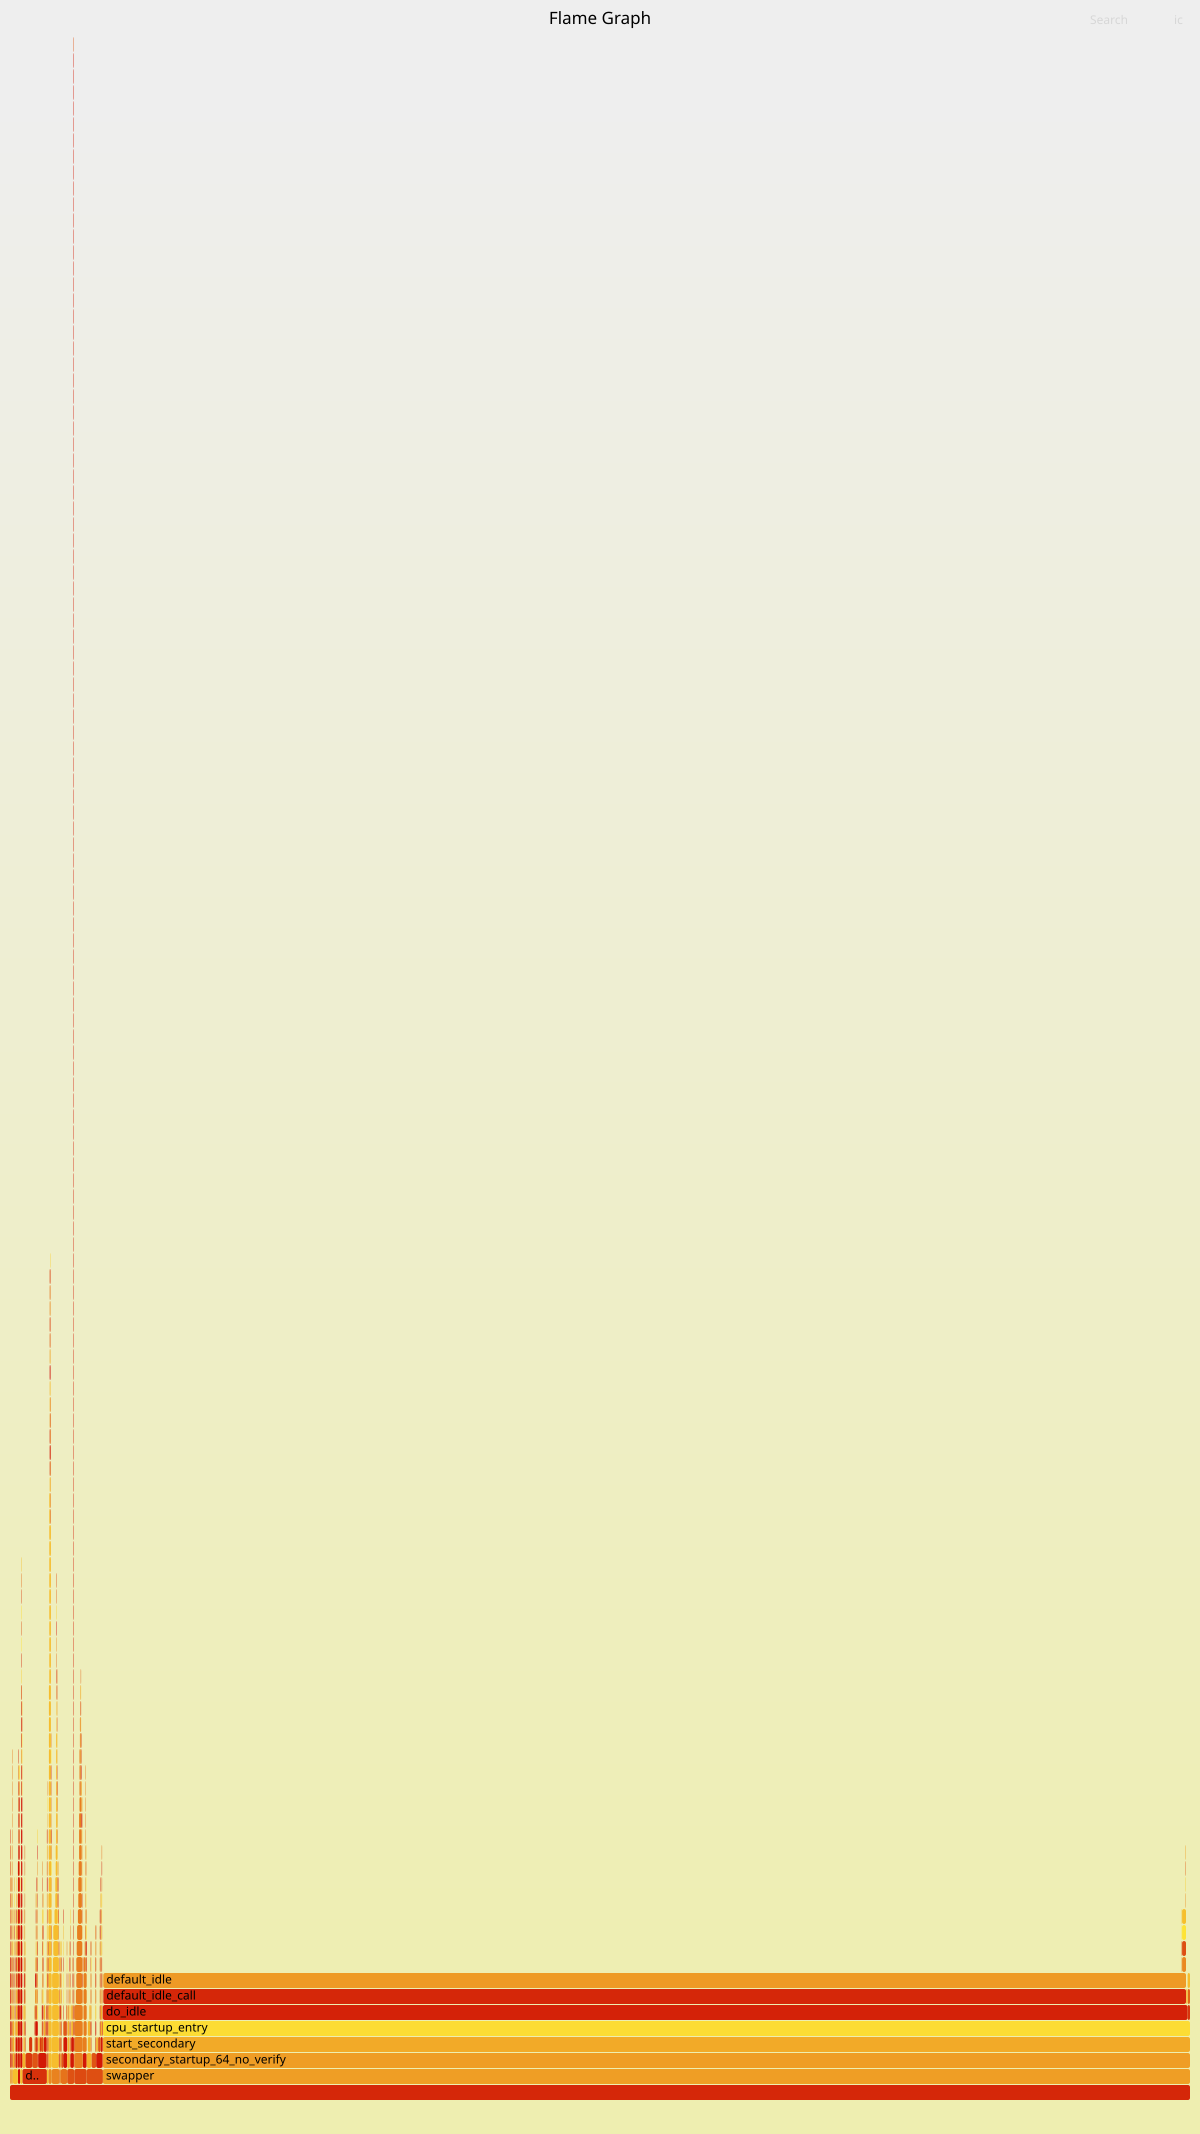
\includegraphics[scale=0.2]{cpu_tricks/6.5.5/V1/flamegraph_20241017_112413.png}
    \caption{Flamegraph illustrating cpuset\_cpus set to CPU 0, and perf instrumenting the rest of the CPUs}
    \label{fig:flamegraph}
\end{figure}


\end{document}  % End of the document